\documentclass[10pt,a4paper,twocolumn]{article}
\usepackage[utf8]{inputenc}
\usepackage{amsmath}
\usepackage{amsfonts}
\usepackage{amssymb}
\usepackage{graphicx}
\usepackage{hyperref}
\usepackage{breqn}
\usepackage{listings}
\usepackage{float}
\usepackage[dutch]{babel}
\author{Ruben Van Assche}
\graphicspath{ {../plots/} }
\title{Data Fitting - Oefening 5}
\date{\today}
\begin{document}
\maketitle
\section{Originele functie}
In de opgave moest de functie $cos(11x)$ op het interval $[0,2 \pi]$. Als eerste kijken we eens naar een plot van deze functie:
\begin{figure}[H]
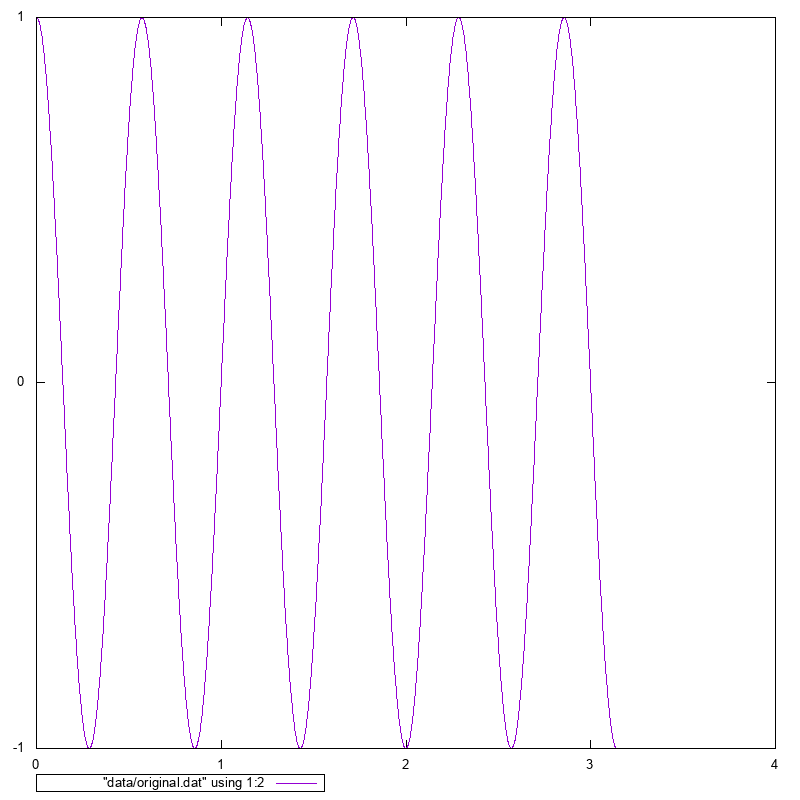
\includegraphics[width=0.4\textwidth]{original-3}
\end{figure}
\subsection{Nulpunten}
Vervolgens kijken we eens naar de nulpunten van deze functie. We weten dat $cos(x)$ als nulpunt $\frac{\pi}{2}$ heeft op het interval  $[0,2 \pi]$. $cos(11x)$ heeft 11 nulpunten op het interval $[0,2 \pi]$. 
$$cos(11x) = 0$$
$$11x = \frac{1}{2} \pi + k \pi$$
$$x = \frac{\pi}{22} +\frac{k \pi}{11}$$
Hierbij is $k = 0,\hdots,10$. Wanneer we dit verder trekken verkrijgen we volgende nulpunten:
$$
\begin{matrix}
\frac{\pi}{22}  &  \frac{\pi}{22} +\frac{\pi}{11} & \frac{\pi}{22} +\frac{2 \pi}{11} \\ 
\frac{\pi}{22} +\frac{3 \pi}{11} & \frac{\pi}{22} +\frac{4 \pi}{11} &  \frac{\pi}{22} +\frac{5 \pi}{11}\\ 
\frac{\pi}{22} +\frac{6 \pi}{11} & \frac{\pi}{22} +\frac{7 \pi}{11}  & \frac{\pi}{22} +\frac{8 \pi}{11} \\
\frac{\pi}{22} +\frac{9 \pi}{11} & \frac{\pi}{22} +\frac{10 \pi}{11} &
\end{matrix}
$$
Of decimaal:
$$
\begin{matrix}
0,1427996661 &  0,4283989982 & 0,7139983304 \\
0,9995976625 & 1,2851969947 & 1,5707963268 \\
1,8563956589 & 2,1419949911 & 2,4275943232 \\
2,7131936554 & 2,9987929875& 
\end{matrix}
$$
\subsection{Extrema}
De extrema van de $cos(x)$ functie zijn -1 en 1. Een aanpassing hiervan kan enkel wanneer een transformatie van de vorm $r*cos(x)$ of $cos(x)+r$ plaatsvindt. Gezien deze niet gebeurt bij de transformatie van $cos(x)$ naar $cos(11x)$ zullen de extrema hetzelfde blijven -1 en 1.
\section{Trigonometrische Interpolant}
Voor het volgende deel van de opgave moest een trigonometrische interpolant bepaald worden. De gegeven punten hiervoor zijn:
$$
\begin{matrix}
\textbf{x} & 0 &  \pi/2 & \pi \\
\textbf{y} & 1 & 0 & -1 \\
\end{matrix}
$$
De bedoeling is om een trigonometrische interpolant van de vorm:
$$\frac{a_{0}}{2} + a_{1}cos(x)+b_{1}sin(x)$$
Hiervoor worden volgende formules gebruikt:
$$a_{j} = \frac{2}{n}\sum^{n-1}_{0}y_{k}cos(jx_{k})$$
$$b_{j} = \frac{2}{n}\sum^{n-1}_{0}y_{k}sin(jx_{k})$$
Wanneer we deze formules invullen met de gegevens komen we volgende coëfficiënten uit:
$$
\begin{matrix}
 & \textbf{a} & \textbf{b} \\
\textbf{0} & 0 &  0 \\
\textbf{1} & 1.33333333 & 0 \\
\end{matrix}
$$
En dus is de trigonometrische interpolant: 
$$1.33333cos(x)$$
Vervolgens plotten we de interpolant met de originele functie:
\begin{figure}[H]
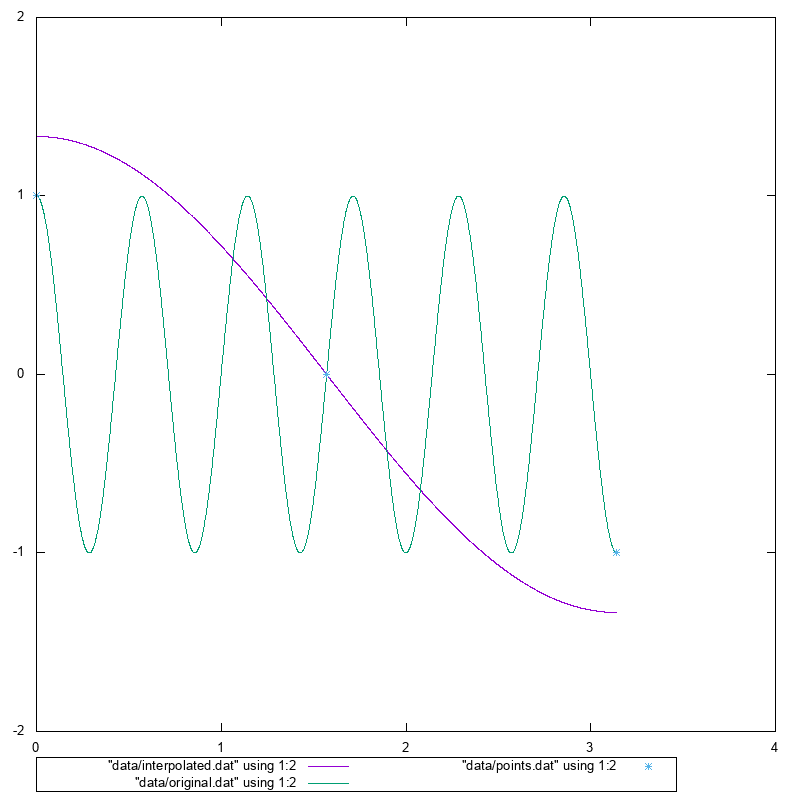
\includegraphics[width=0.4\textwidth]{combined-3}
\end{figure}
Dit komt natuurlijk niet in de buurt van een goede interpolant, in feite is het zelfs geen interpolant. Wanneer we de gegeven punten en de interpolant plotten zien we dat deze niet door de originele punten gaat:
\begin{figure}[H]
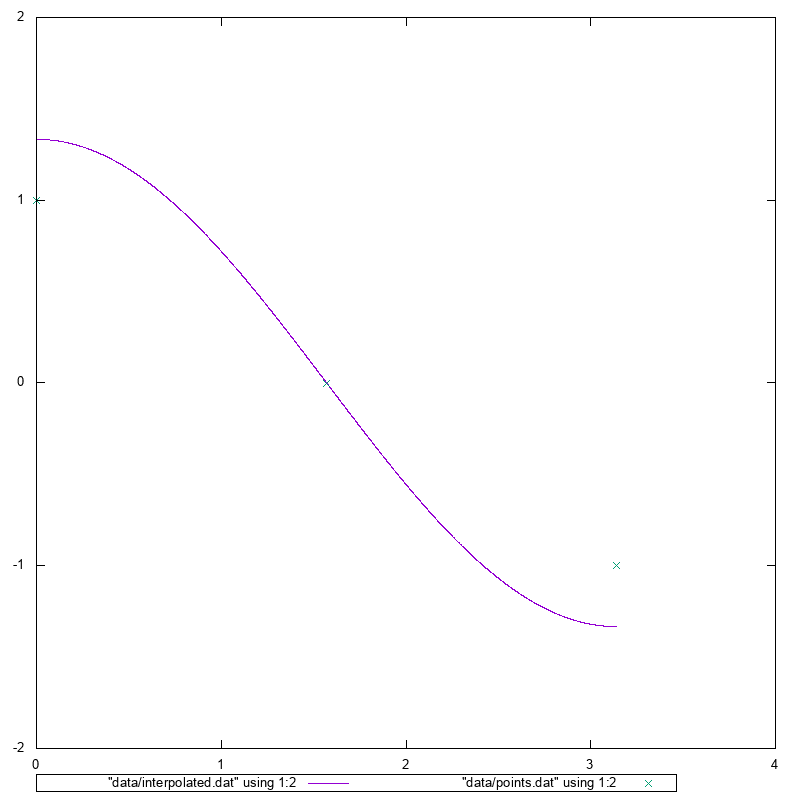
\includegraphics[width=0.4\textwidth]{interpolated-3}
\end{figure}
\section{Discrepantie}
Er is duidelijk iets mis met de interpolatie. Deze gaat slechts door één punt $(\frac{\pi}{2}, 0)$ inplaats van alle en volgt totaal niet de vorm van de originele functie.

\subsection{Oplossing}
\subsubsection{Algoritme}
Een eerste idee kan natuurlijk zijn dat er ergens een foutje is geslopen in het vertalen van de theorie naar de code, nu is dit zeer snel gecheckt. Wanneer de gegevens van de voorbeelden in de theorie worden ingevuld in het algoritme. Dan zien we dat deze dezelfde resultaten als in de theorie opleveren. Dus kunnen we feitelijk stellen dat het algoritme klopt.
\subsubsection{Periodiciteit}
Wat belangrijk is voor de trigonometrische interpolant is dat de de datapunten gelijk verdeeld zijn over het interval $2\pi$ anders krijgen we dus een fout zoals deze. Dit zien we door een extra punt $(\frac{3}{2})\pi, 0)$ toe te voegen. Dan verkrijgen we volgende plot:
\begin{figure}[H]
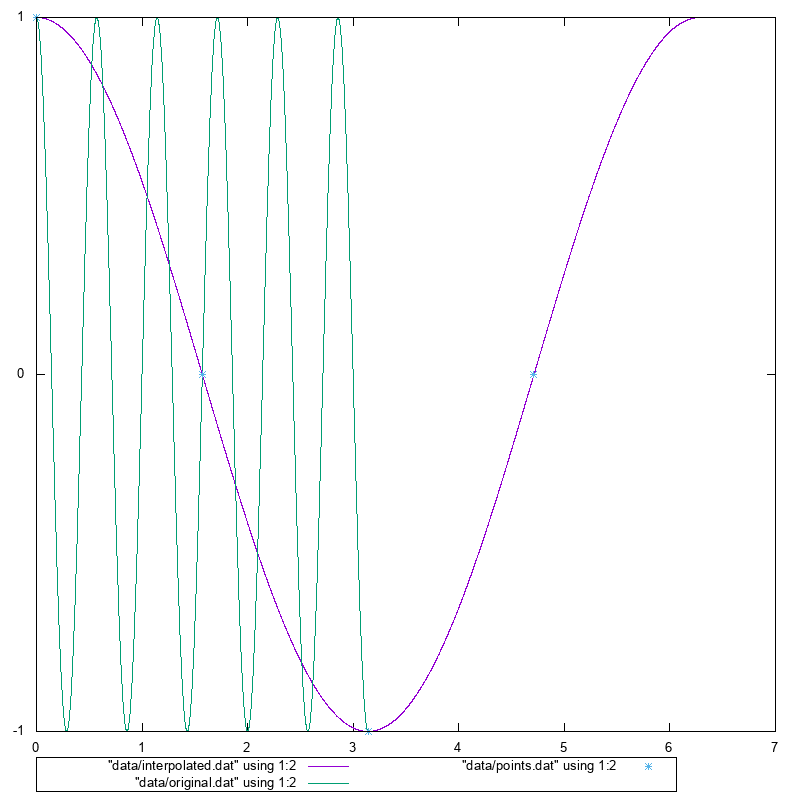
\includegraphics[width=0.4\textwidth]{combined-4}
\end{figure}
Dit begint er al beter uit te zien! De interpolant gaat nu door de 4 punten en haar extrema blijven ook binnen het berekende interval $[-1, 1]$ van de originele functie.
\\
\\
Nu kunnen we niet altijd zomaar een extra punt toevoegen. Een verstandiger idee is om de punten te transformeren van het interval $[0,\frac{3}{2}\pi]$ naar $[0, 2\pi]$. Hierbij is de eindwaarde van het originele interval $\frac{3}{2} \pi$ inplaats van $\pi$. Dit omdat het laatste punt niet gelijk mag zijn aan het eerste punt. Vervolgens gebruiken we volgende formule:
$$x = \frac{2 \pi}{d-c}(s-c)$$
Hierbij schalen we de originele punten s van $[c, d]$ naar $[0, 2\pi]$. In dit geval is dus $c = 0$ en $d = \frac{3}{2}\pi$. Wat volgende transformatie oplevert:
$$ x = \frac{2\pi}{0-\frac{3}{2}\pi}(s-0) = \frac{4}{3}s$$
Dit levert dan volgende punten op:
$$
\begin{matrix}
\textbf{x} & 0 & \frac{2}{3} \pi & \frac{4}{3}\pi \\
\textbf{y} & 1 & 0 & -1 \\
\end{matrix}
$$
Wanneer we vervolgens de interpolant berekenen krijgen we volgende functie:
$$cos(x) + 0.577350sin(x)$$
Dit geplot geeft volgend resultaat:
\begin{figure}[H]
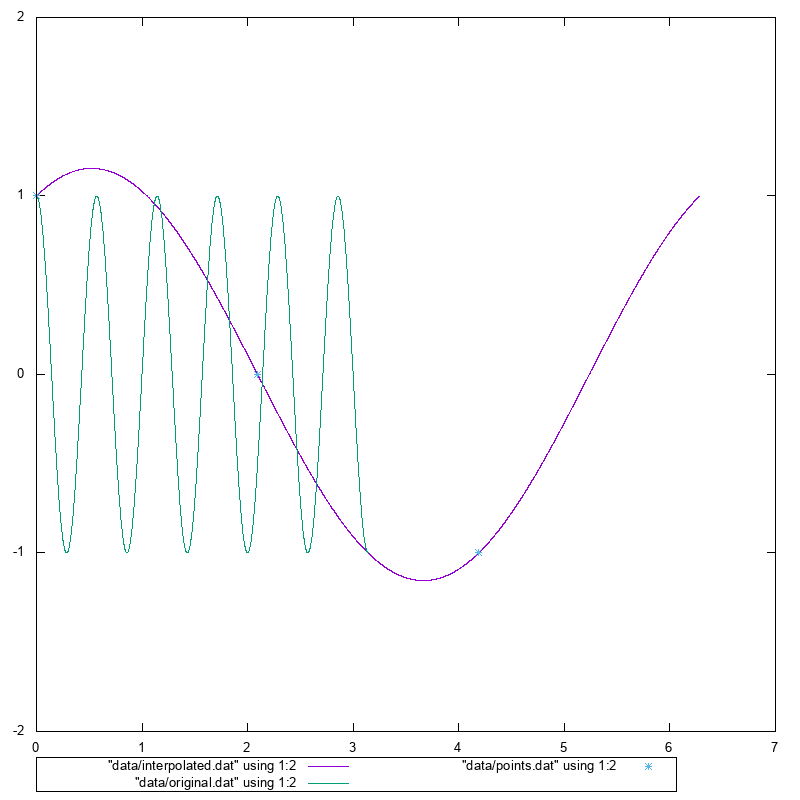
\includegraphics[width=0.4\textwidth]{combined-transformed}
\end{figure}

\subsubsection{De vorm}
Er is nog steeds iets mis met de interpolatie, de vorm is niet juist! Nu is dit niet geheel onlogisch: gezien er geen transformatie van $cos(x)$ naar $cos(rx)$ gebeurt. Dit is dan ook niet mogelijk gezien die r afhangt van de keuze van m(in dit voorbeeld = 1). 
\\
\\
We gaan het aantal gegeven punten(n) aan de interpolatie verhogen zodat we uiteindelijk de waarde (m) kunnen verhogen. Dit is niet een echte oplossing gezien dat we extra punten toevoegen terwijl we waarschijnlijk enkel de gegeven punten hebben gekregen.
\\
\\
Momenteel is $n = 3$ en $m = 1$. Volgende condities zijn nodig voor een interpolatie : $2m + 1  = n$ en $2m = n $. Uiteindelijk willen we 11 nulpunten dus hebben we een functie van de vorm $cos(11x)$ nodig. Wat dan weer vereist dat $m = 11$ en dus $n = 22$ of $n = 23$. We kijken eerst naar het geval met $n  = 22$ dit levert volgende interpolant op:
\begin{dmath}
0.090909cos(1x) + 0.090909cos(3x) + 0.090909cos(5x)+ 0.090909cos(7x) + 0.090909cos(9x) + 0.522727cos(11x)
\end{dmath}
Wanneer we deze interpolant plotten zien we dat deze de vorm volgt van de originele functie!
\begin{figure}[H]
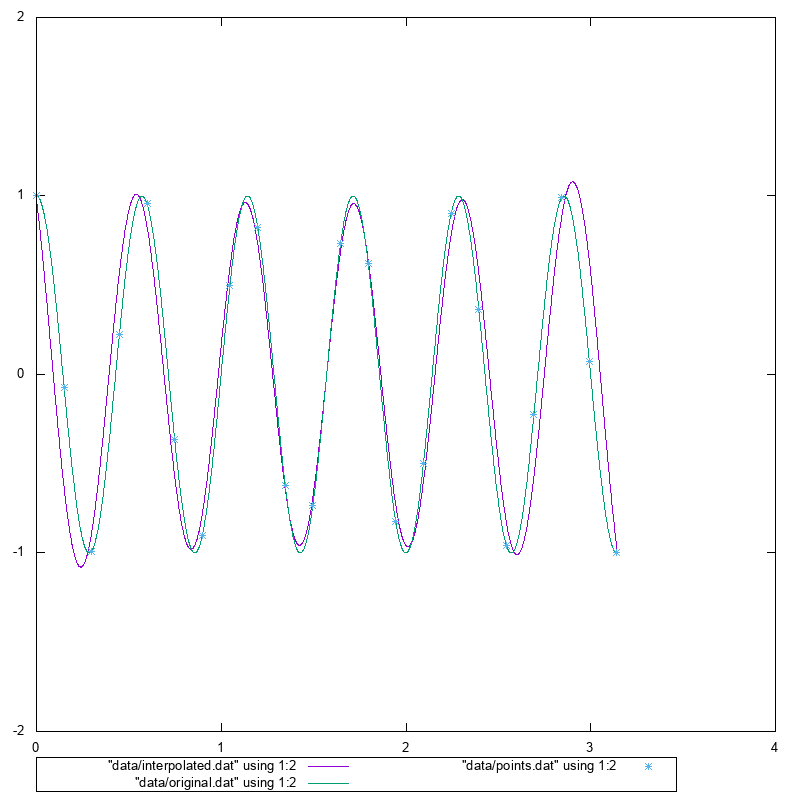
\includegraphics[width=0.4\textwidth]{combined-22}
\end{figure}
Maar dit is nog geen goede interpolant want de functie gaat niet door alle originele datapunten en haar beeld ligt niet in $[-1, 1]$. We kijken naar de interpolant met $n = 23$ welke volgende functie oplevert:
\begin{dmath}
0.086957cos(1x) + 0.086957cos(3x) + 0.086957cos(5x) + 0.086957cos(7x) + 0.086957cos(9x) + 1.043478cos(11x)
\end{dmath}
Wanneer we de plot bekijken zien we dat het interval van het beeld een stuk geworden dan de versie met $n = 22$.
\begin{figure}[H]
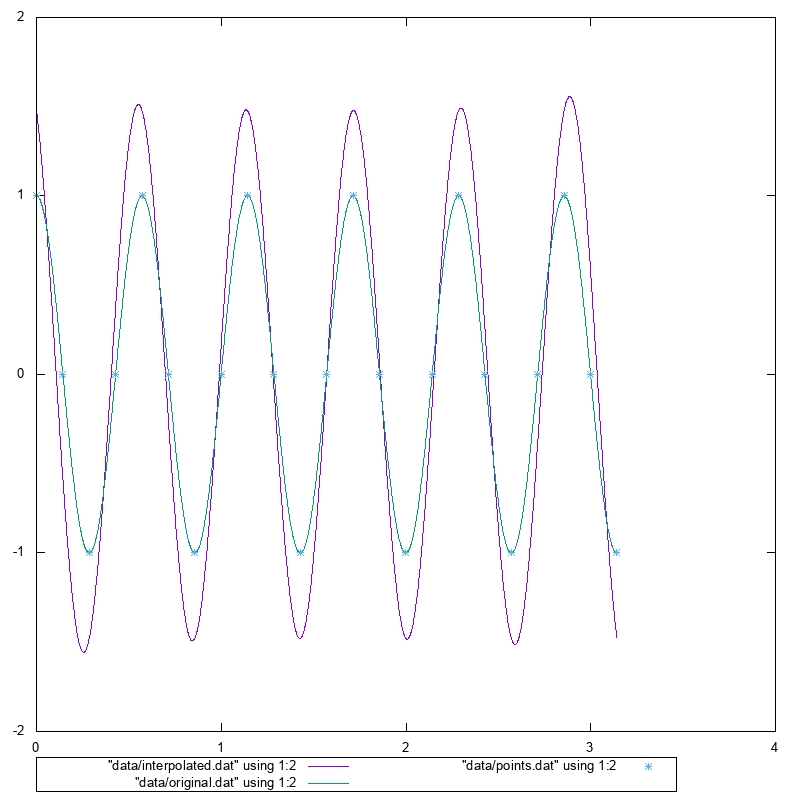
\includegraphics[width=0.4\textwidth]{combined-23}
\end{figure}
\subsubsection{Een combinatie}
We hebben voor deze discrepantie 2 oplossingen gezien, uiteindelijk zal de oplossing een combinatie van beide zijn. Bij $n = 22$ zullen we de punten transformeren met $x = \frac{42}{22}s$. Dit ratio $ \frac{42}{22}$ halen we uit volgende formule:
$$ \frac{(n-1)*2}{n}$$
Uiteindelijk bekomen we als interpolant:
\begin{dmath}
0.710858cos(6x) + 0.615962sin(6x) + 0.174734cos(7x) + 0.112295sin(7x) + 0.119972cos(8x) + 0.054790sin(8x) + 0.101026cos(9x) + 0.029664sin(9x) + 0.093146cos(10x) + 0.013392sin(10x) + 0.045455cos(11x)
\end{dmath}
En dit geeft een mooie plot:
\begin{figure}[H]
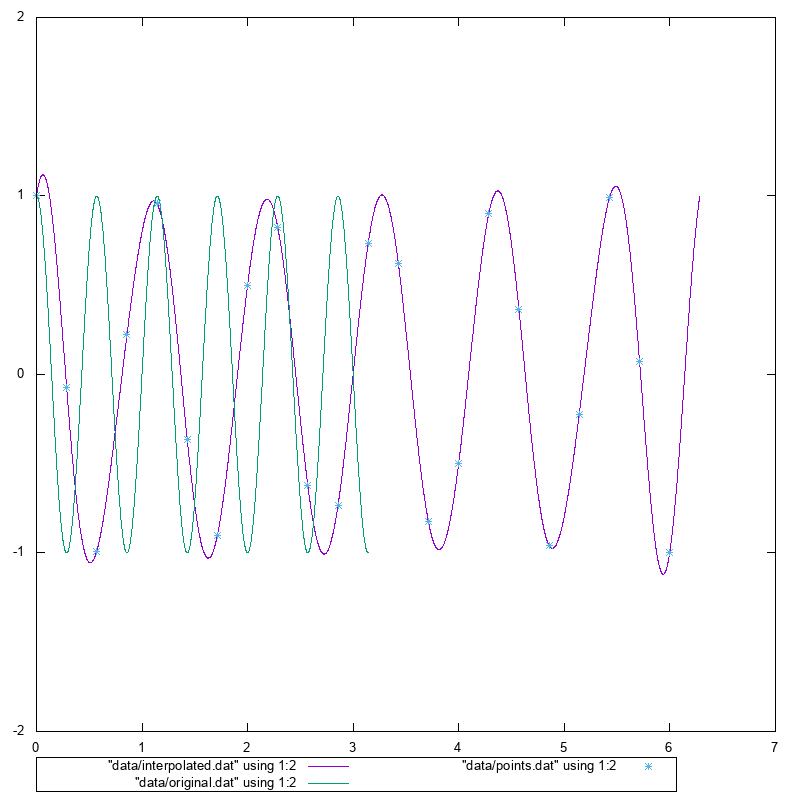
\includegraphics[width=0.4\textwidth]{combined-22-transformed}
\end{figure}
Dit process herhalen we ook bij $n = 23$ waarbij de punten getransformeerd worden met $x = \frac{44}{23}s$:
\begin{dmath}
0.680593cos(6x) + 0.635630sin(6x) + 0.173311cos(7x) + 0.122336sin(7x) + 0.118872cos(8x) + 0.061595sin(8x) + 0.099528cos(9x) + 0.035372sin(9x) + 0.090881cos(10x) + 0.018885sin(10x) + 0.087365cos(11x) + 0.005976sin(11x)
\end{dmath}
Dit levert dan volgende plot op:
\begin{figure}[H]
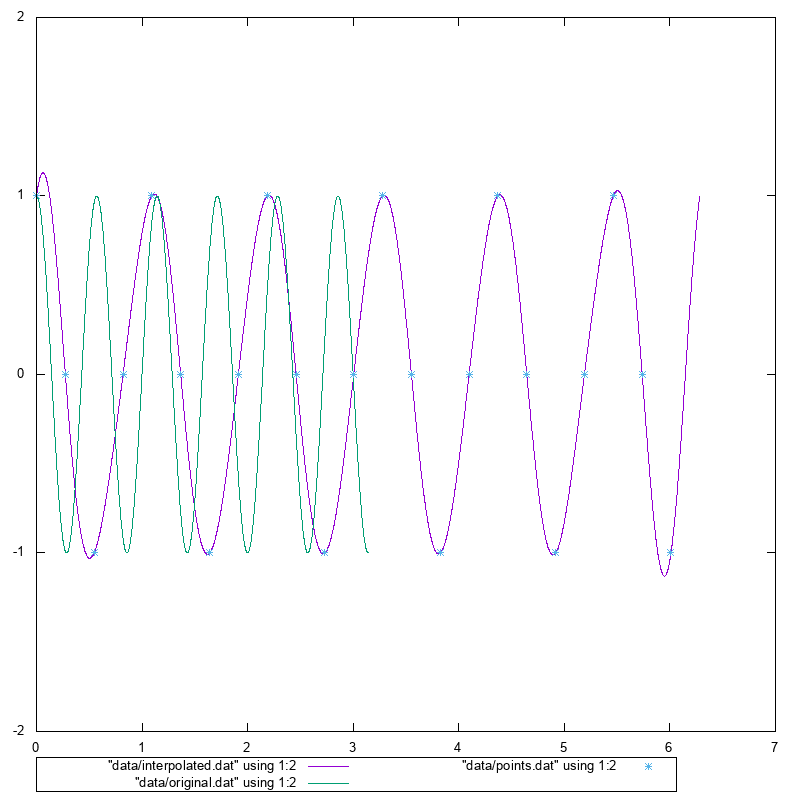
\includegraphics[width=0.4\textwidth]{combined-23-transformed}
\end{figure}
Wat snel opvalt is dat nu het beeld van de interpolant wel veel meer in het interval $[-1, 1]$ ligt t.o.v. $n = 22$.
\\
\\
Als laatste herschalen we $p(x)$, de interpolant terug naar $[0, \pi]$. Dit doen we door $p(x)*(\frac{22}{42})$ uit te voeren bij $n = 22$ en $p(x)*(\frac{23}{44})$ bij $n = 23$. Voor $n  = 22$ levert dit volgende plot op:
\begin{figure}[H]
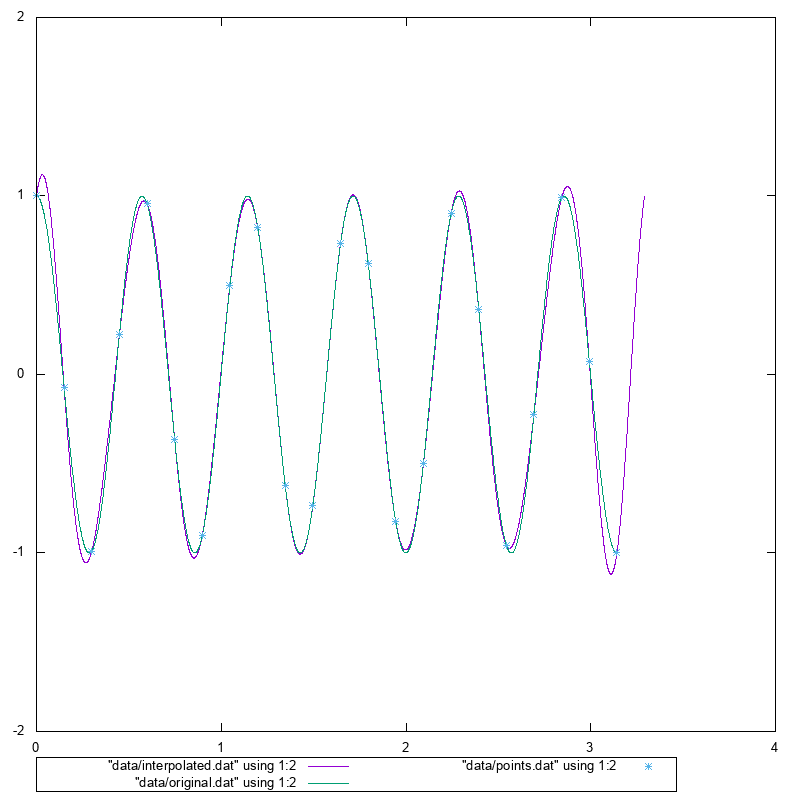
\includegraphics[width=0.4\textwidth]{combined-22-transformed-scaled}
\end{figure}
Als laatste kijken we naar een herschaalde plot van $n = 23$:
\begin{figure}[H]
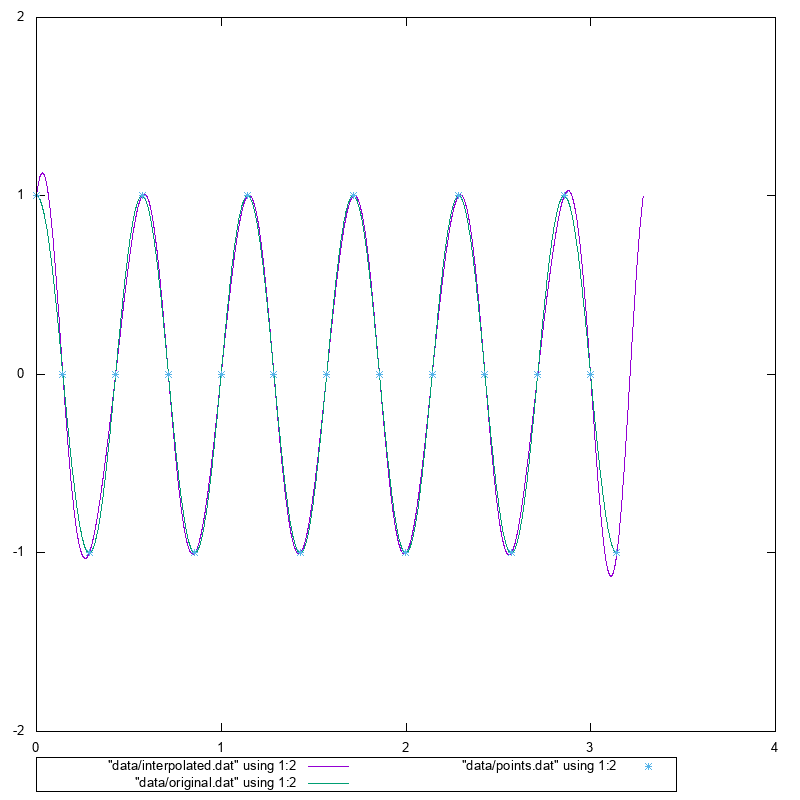
\includegraphics[width=0.4\textwidth]{combined-23-transformed-scaled}
\end{figure}
Dit is waarschijnlijk het beste wat we in de buurt gaan komen van een interpolant die $cos(11x)$ benadert. De functie loopt door de gegeven punten, volgt de vorm en haar beeld blijft ongeveer in het interval $[-1, 1]$
\section{Code}
Nog een klein woordje over de code: normaal schrijf ik veel stukken zodat elke mogelijke oplossing telkens bij het runnen wordt gegeneerd. Deze keer heb ik vaak zoveel liggen aanpassen dat het me interessanter leek om sommige regels soms niet te laten compileren. Ik heb steeds bij deze regels een stuk commentaar geschreven over wat ze doen indien ze toch worden gecompileerd.
\end{document}